\documentclass{article}
\usepackage[legalpaper, margin=1in]{geometry}
% \usepackage[utf8]{inputenc}

\usepackage{hyperref}

\usepackage{graphicx}
\graphicspath{ {./pics/} }

\title{ECE 3 Project Report}
\author{Joseph Picchi\\
UID: 605-124-511}
\date{}

\begin{document}

\maketitle

\section{Develop}
\label{section:Develop}

I first decided to collect sensor calibration data in the room in which I would be runnning my car on race day, and I extracted the minimum value for each sensor, maximum value for each sensor, and the sensor weighting scheme from my calibration data for use in my Energia code.

Next, I decided to implement a basic version of my code that uses only a proportional controller to follow a straight-line path from beginning to end without stopping or performing a doughnut, continually modifying the numerical constants in my code (e.g. base motor speed, \(K_p\), and \(K_d\)) until the car was able to perform this simplified task successfully.

Afterwards, I added the functionality of a doughnut turn at the end of the straight track and a full stop once the car returned to the start position, which required tuning of the encoder count threshold that the car should surpass before terminating the doughnut procedure; I decided to move on to the next step once both the doughnut and stop were successful in every trial run.

Next, I replaced the straight track with the actual track (i.e. the curvy race day track), and I added a derivative control element in addition to the proportional control element, continually fine-tuning the base speeds, \(K_p\) and \(K_d\) values, and the maximum change in wheel speed so that the car could handle large turns at a quick pace; I decided to move on once my car was able to make a round-trip successfully in under 12 seconds for a majority of trials when the car started out with the track centered underneath the sensor array.

Lastly, I edited the code to ensure that the car could start successfully from any of the 4 start positions, reducing the base speed and creating custom \(K_p\) and \(K_d\) values for the first 1 second of forward movement to ensure that the car would center itself along the track before picking up speed; I decided that the code no longer needed improvement once the majority of trials from each start position resulted in successful trips in under 12 seconds.

\section{Conduct}

\begin{itemize}
    \item The variables I controlled were (1) the amount of ambient lighting in the room (the room in which the car ran had no windows), (2) the speeds to which the motors were set when the car performed a doughnut, (3) the number of encoder counts waited until the doughnut procedure finished, (4) the minimum value for each sensor (from the sensor calibration data), and (5) the maximum value for each sensor (from the sensor calibration data).
    
    \item The variables I measured (i.e. experimentally altered across different trials) were (1) the pwm base speed of the motors, (2) the \(K_p\) constant, (3) the \(K_d\) constant, (4) the weighting scheme used to fuse the sensor values, (5) the start position of the car, and (6) the maximum pwm speed change (i.e. the maximum pwm value added or subtracted) from the base speed of the left and right motors.
    
    \item The first test that I performed was running the car at a very slow base speed (i.e. a pwm value of 30) with a strictly proportional controller, 8-4-2-1 weighting scheme, max speed correction value of 50 pwm, and a start position of 1; the car was able to complete the track slowly.
    
    \item The second test that I performed was to again run the car at a very slow base speed, but this time with a derivative control element added in addition to the propertional controller (i.e. \(K_d\) was changed from being zero-valued to nonzero-valued).
    
    \item The third test that I performed was to increase the base speed significantly (from a pwm value of 30 to a pwm value of 80), keeping the same 8-4-2-1 weighting scheme while attempting to tune the \(K_p\), \(K_d\), and maximum pwm speed change values so that the car would not leave the track; this was unsuccessful because I was unable to get the car to stay on the track without adding additional features to the code.
    
    \item The fourth test was to alter the sensor fusion weighting scheme, the \(K_p\) value, the \(K_d\) value, and the maximum speed change value so that the car would not leave the track; this was again unsuccessful.
    
    \item The fifth test was to increase the maximum change in motor speed (i.e. the maximum pwm value by which the left and right motor speeds can change relative to their base values) and to edit the implementation so that whenever the newly-calculated, error-informed motor speed for either motor was less than 0, that motor would be set to spin in reverse; altering \(K_p\), \(K_d\), and the sensor weighting scheme thereafter enabled consistently successful runs with runtimes of under 12 seconds when the car started at start position 1.
    
    \item The sixth test was to start the car at each of the 4 starting positions (not just position 1, which was the start position in all of the previous tests), which required alteration of the code so that the base speed was very slow and derivative control was disabled for the first 1 second of forward movement, giving the car time to slowly center itself over the middle of the track before picking up speed.
    
    % \item The first test that I ran was running the car on the straight track from beginning to end (without a dougnut or stop procedure) after I had already implemented the sensor fusion procedure with a proportional controller (\(K_p = 0.5\)) and slow base speed (40 pwm).
    
    % \item The next test that I ran was running the car on the straight track and stopping once the car detects the end of the track, keeping the same controller and base speed parameters as the previous test.
    
    % \item The third test was running the car on the straight track and performing a doughnut once the car detects the end of the track, setting the left and right motors to spin in opposite directions at a pwm speed of 100, and tuning the number of encoder counts to wait until the doughnut procedure is finished (ultimately settling on the value of 380 encoder counts).
    
    % \item The fourth test was running the car on the straight track, performing a doughnut at the end of the track, and stopping once the car returns back to the starting position.
    
    % \item The fifth test 
    
    
\end{itemize}

\section{Analyze}

\subsection{Test Logs}

\begin{center}
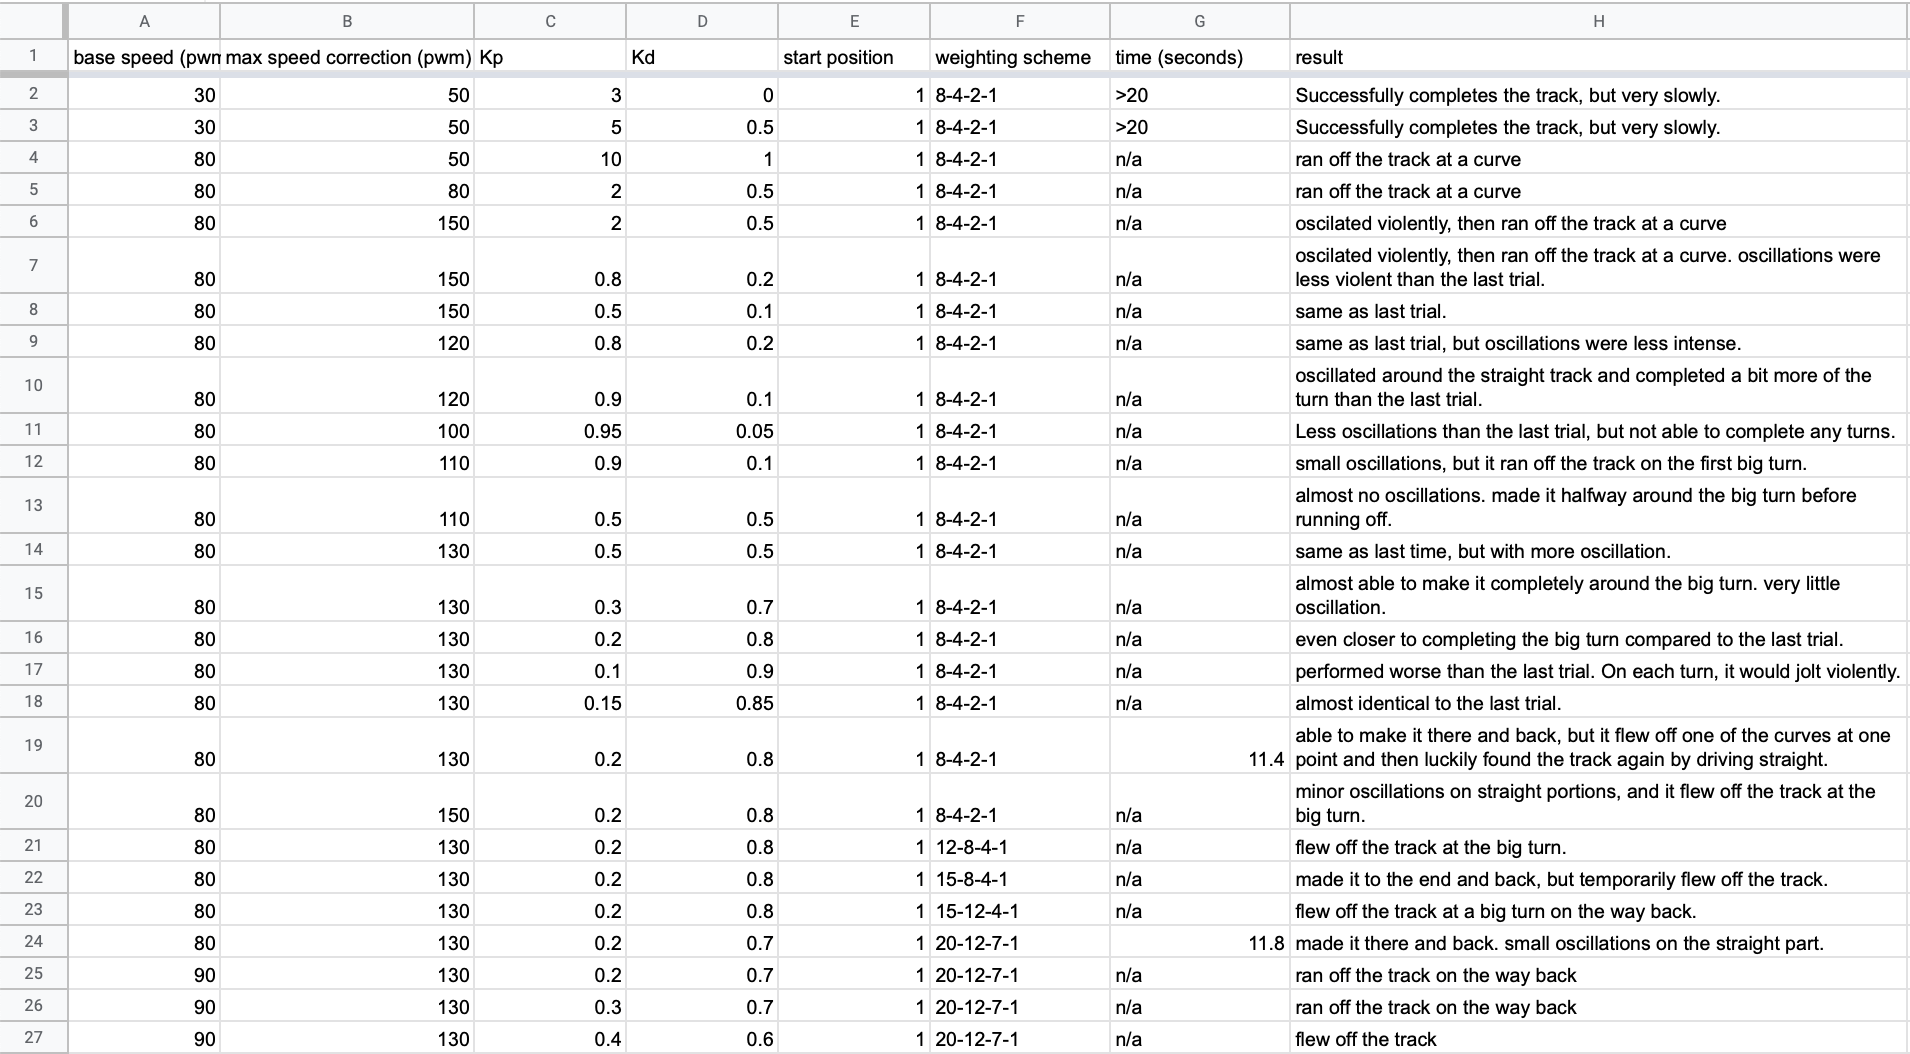
\includegraphics[scale=0.45]{pics/log1.png} \\
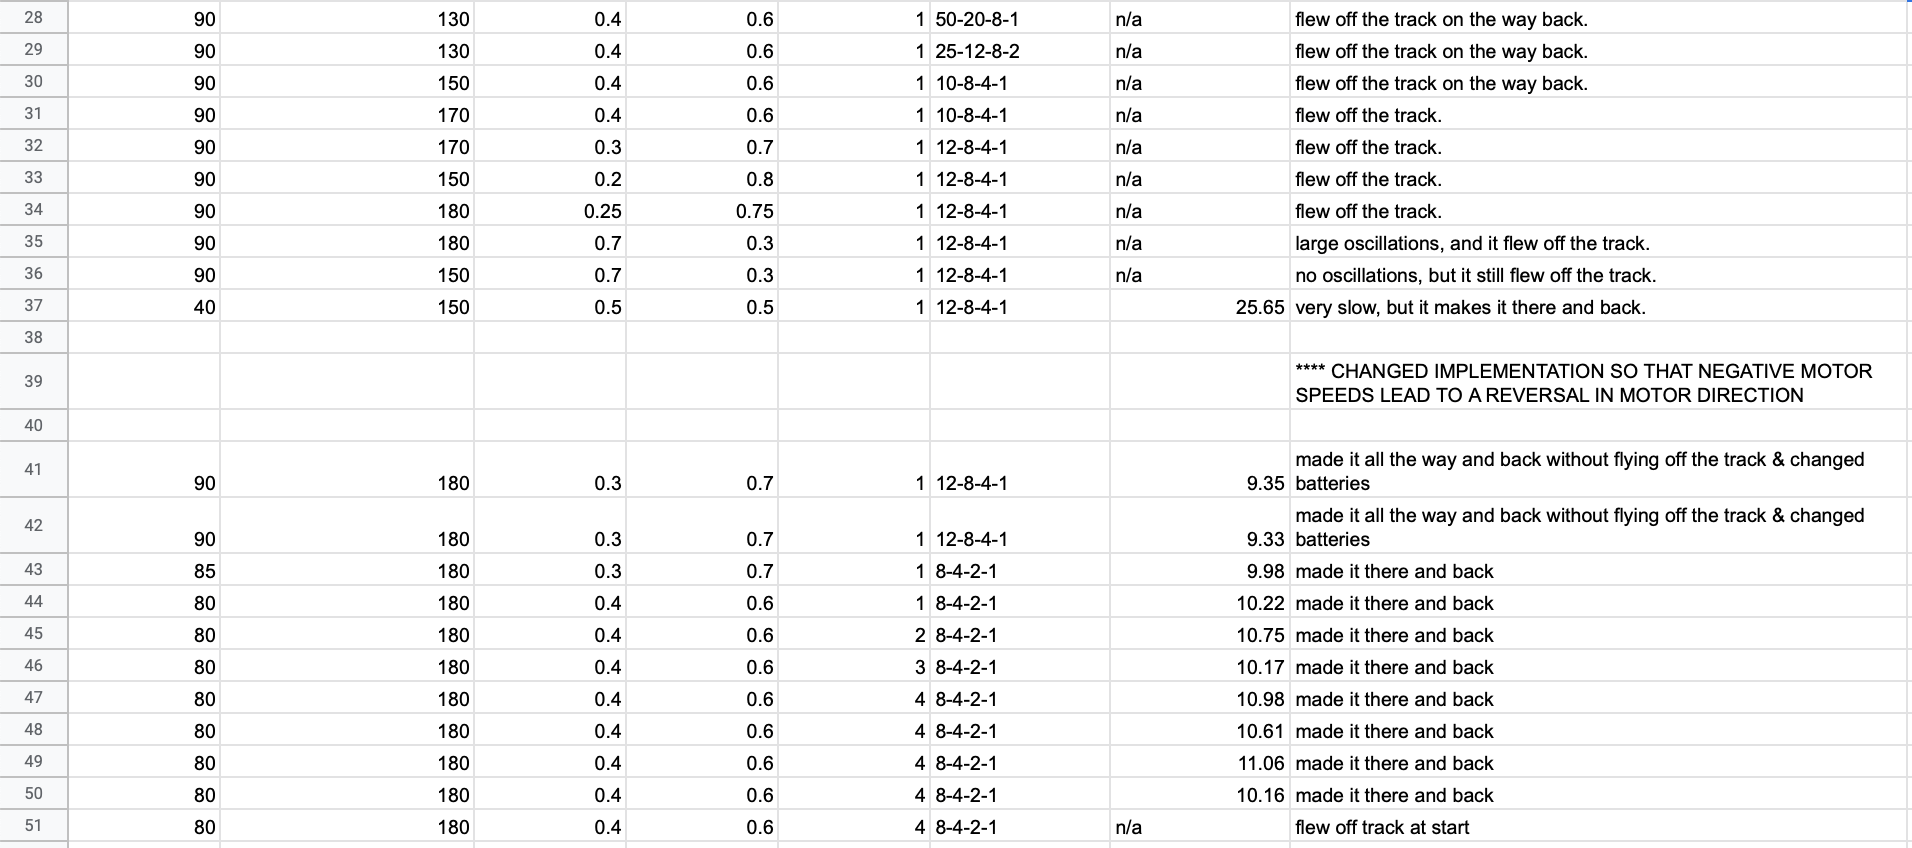
\includegraphics[scale=0.45]{pics/log2.png} \\
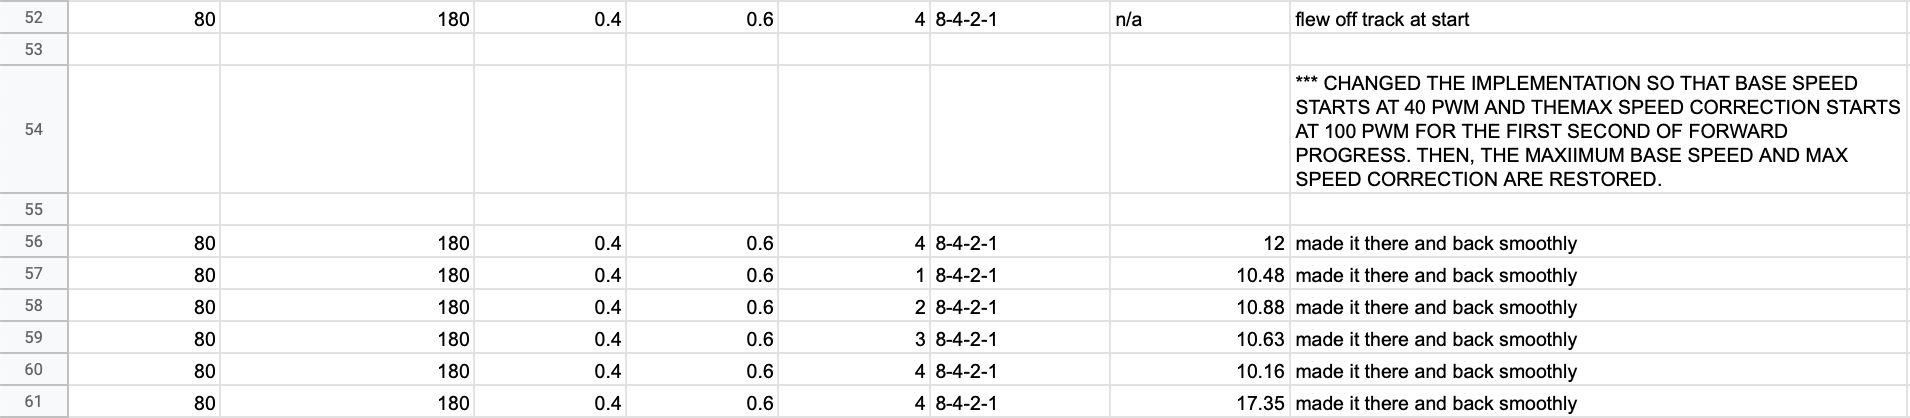
\includegraphics[scale=0.45]{pics/log3.png}
\end{center}
\noindent \textbf{Figure 1:} Table of test logs for all trials conducted (with indications of how and when the code was altered). The spreadsheet of test logs is available at this \underline{\href{https://docs.google.com/spreadsheets/d/1jPR7GRYgVLwytfdNqy9U_3dGLSMvrA-QAdmIjt_J-6s/edit?usp=sharing}{link}}.


\subsection{Calibrated Sensor Data}
\begin{center}
    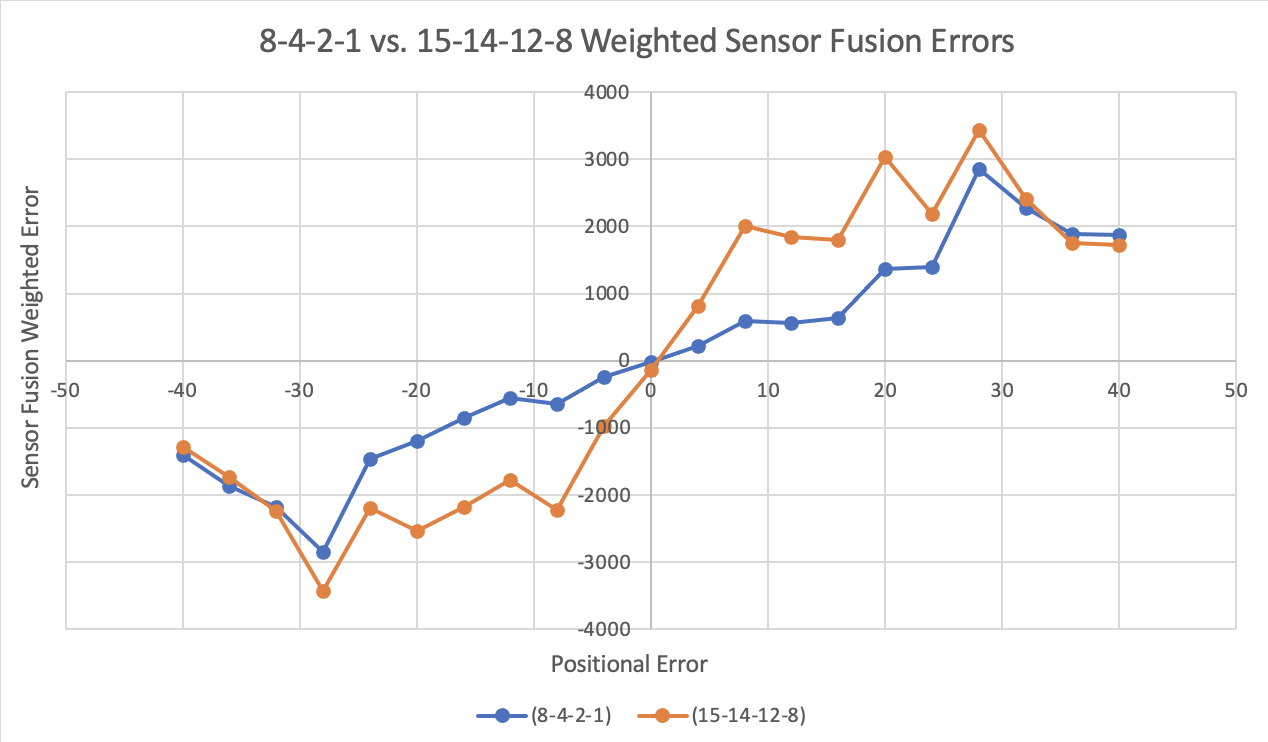
\includegraphics[scale=0.5]{pics/sensor_fusion_new.png}    
\end{center}

\noindent \textbf{Figure 2:} Visualization of the sensor fusion weighting schemes from calibrated sensor data. Calibrated sensor data was collected in the environment in which the car would run on race day (i.e. my bathroom). Numerical sensor errors are normalized and weighted with 8-4-2-1 and 15-14-12-8 weighting schemes, and the resulting sensor fusion weighted errors are plotted against the positional error of the track relative to the car's sensor array.

\subsection{Dependence of Track Completion Time on Start Position}
\begin{center}
    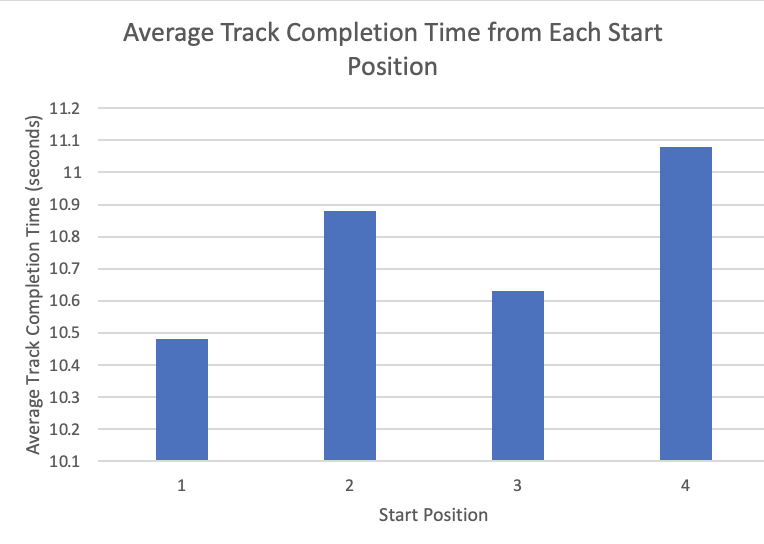
\includegraphics[scale=0.7]{pics/completion_times.png}    
\end{center}

\noindent \textbf{Figure 3:} Plot of the average amount of time required for the car complete the entire track when it started at each of the 4 starting positions. This figure only considers trials that were performed after all features of the code had already been introduced.


%------------------------------------------------------------------------
\section{Interpret}

\begin{itemize}
    \item \textbf{Figure 1:} The test logs can be conceptually divided into 3 main stages of development that correspond to the introduction of new features in the code: (1) running the car successfully at slow speeds and failing to complete successful trials at fast speeds, (2) successfully running trials in under 12 seconds from start position 1 due to tuned \(K_p\) and \(K_d\) values, as well as the added feature of reversed motor speeds (described in the "Conduct" section and in the test logs themselves), and (3) successfully running trials in under 12 seconds from all 4 start positions, which was achieved by setting a low base speed and custom \(K_p\) and \(K_d\) values for the first 1 second of forward movement.
    
    \item \textbf{Figure 2:} The 8-4-2-1 weighting scheme produces a gradual rise in error value as the car deviates slightly from the center of the path, increasing that error value sharply as the path nears the edge of the sensor array so as to encourage a strong correction in motor speed when the car is far away from the center of the path; in contrast, the 15-14-12-8 weighting scheme produces a sharp rise in error value for small deviations from the path, which encourages more drastic motor speed corrections when the car is only slightly off-center.
    
    \item \textbf{Figure 3:} The car completed the track in the fastest time when it was placed at starting position 2 because position 2 was the most centered over the middle of the track, and the car completed the track in the slowest time when it was placed at starting position 4 because position 4 was furthest from the center of the track, thus forcing the car to spend more time correcting its position at the beginning of trials in which it was placed at position 4.
    
\end{itemize}

\end{document}
